\chapter{Framework Valutati}
	Il primo passo necessario nella valutazione di questi framework è stato 
	chiarire bene il fine del loro impiego. Durante la fase di ricerca abbiamo 
	notato una gran confusione nell'attribuire a ciascun framework il tipo di
	applicazione che permetteva di realizzare. Spesso il fatto che 
	l'applicazione venisse eseguita all'interno di una componente nativa veniva 
	pubblicizzato come se il framework fosse in grado di creare una completa 
	applicazione nativa (anziché ibrida); in altri casi 
	veniva confuso il concetto di \crosscomp 
	(\hyperref[sec:nativapp]{vedi~\ref{sec:nativapp}}) con quello di 
	applicazione ibrida; in altri ancora non veniva mostrata la separazione 
	concettuale che vi è tra framework utili per la sola costruzione della 
	logica e dell'interfaccia grafica dell'applicazione e framework che 
	permettono d'incapsulare il contenuto web in una componente nativa creando 
	così un'applicazione ibrida.
	
	Allo scopo di dare ordine per descrivere al meglio le differenze tra i vari 
	framework abbiamo ritenuto opportuno suddividerli a seconda del tipo di 
	applicazioni che sono in grado di produrre.
	
	Abbiamo così classificato Titanium Appcelerator come framework per la 
	realizzazione di applicazioni native; Phonegap/Cordova, Rho Mobile e Sencha 
	Touch come quelli dediti alla creazione di applicazioni ibride; jQuery 
	Mobile, KendoUI Mobile e PhoneJS utili per implementare complete 
	applicazioni web e per la logica e l'interfaccia grafica di applicazioni 
	ibride.

	\section{Framework per Applicazioni Native}
		
		\subsection{Titanium Appcelerator}
		\label{sec:titanium}
			Titanium è una piattaforma gratis e open source di sviluppo di 
			applicazioni mobili che permette la creazione di applicazioni native
			\crossplat{} per iOS, Android, BlackBerry e Tizen usando il 
			linguaggio JavaScript. Usando JavaScript e HTML è anche possibile
			creare semplici applicazioni Web.
			
			Titanium agisce come un ponte tra i sistemi operativi nativi e il 
			codice dell'applicazione. La figura \ref{fig:ti_stack} illustra 
			questa architettura.
			\begin{figure}[h]
				\centering
				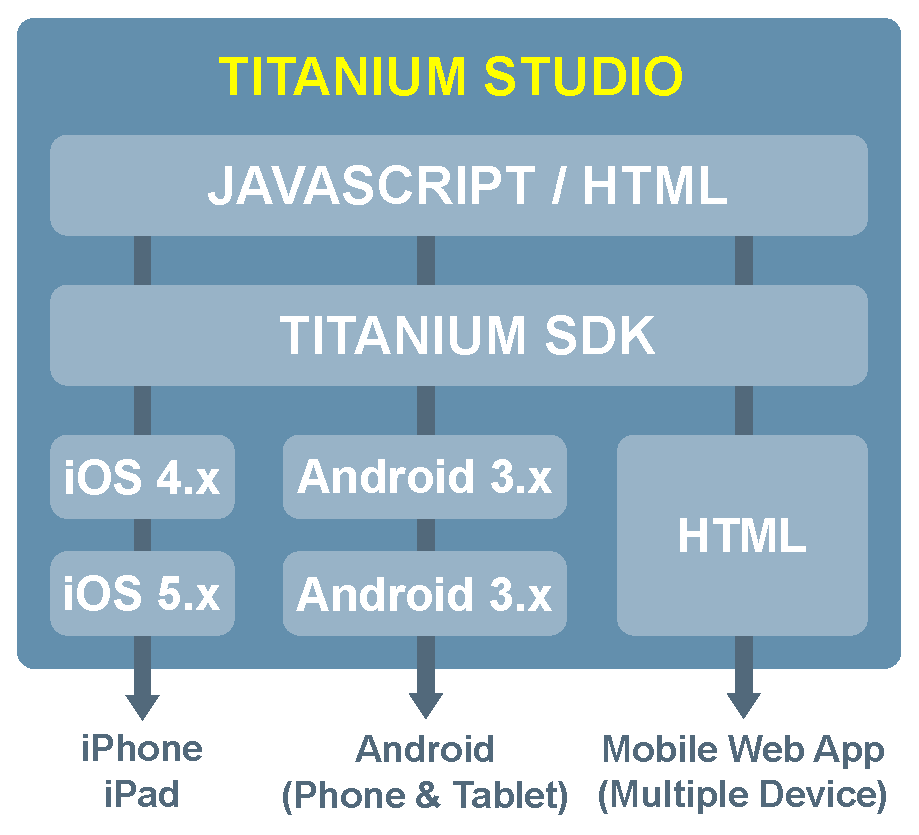
\includegraphics[keepaspectratio=true, width=12cm]{titanium-stack.eps}
				\caption{
					Architettura nello sviluppo di un applicazione \crossplat{} 
					mediante Titanium Studio.
				}
				\label{fig:ti_stack}
			\end{figure}
			In fondo alla pila si trova il sistema 
			operativo di destinazione: Android, iOS o il browser (per quanto 
			riguarda le applicazioni web); sulla cima troviamo il codice 
			dell'applicazione scritta in JavaScript e in mezzo trova posto
			Titanium SDK insieme alle proprie APIs. Utilizzando tali interfacce 
			nella propria applicazione è possibile fare azioni come mostrare la 
			fotocamera,	aprire nuove finestre, disegnare pulsanti, ecc. 
			
			Titanium è descritto come un framework \crosscomp{}\citep{Web:peptechlearn.blogspot.it} anche se l'uso che si fa di 
			questo appellativo in questo caso non è del tutto corretto. Come 
			spiega lo stesso amministratore delegato di Appcelerator Inc., Jeff 
			Haynie, in un intervento online su 
			\mbox{stackoverflow.com}\footnote{In quell'occasione era stato 
			chiesto proprio come Titanium potesse funzionare riguardo alla 
			creazione del codice nativo. L'intera discussione è consultabile 
			all'indirizzo 
			\url{http://stackoverflow.com/questions/2444001/how-does-appcelerator-titanium-mobile-work}}
			il modo di operare di Titanium è il seguente:
			\begin{quotation}
				Titanium takes your Javascript code, analyzes and preprocesses 
				it and then pre-compiles it into a set of symbols that are 
				resolved based on your applications uses of Titanium APIs. From 
				this symbol hierarchy we can build a symbol dependency matrix 
				that maps to the underlying Titanium library symbols to 
				understand which APIs (and related dependencies, frameworks, 
				etc) specifically your app needs. I'm using the word symbol in a 
				semi-generic way since it's a little different based on the 
				language. In iPhone, the symbol maps to a true C symbol that 
				ultimately maps to a compiled .o file that has been compiled for 
				ARM/i386 architectures. For Java, well, it's more or less a 
				.class file, etc. Once the front end can understand your 
				dependency matrix, we then invoke the SDK compiler (i.e. GCC for 
				iPhone, Java for Android) to then compile your application into 
				the final native binary.
				
				So, a simple way to think about it is that your JS code is 
				compiled almost one to one into the representative symbols in 
				nativeland. There's still an interpreter running in interpreted 
				mode otherwise things like dynamic code wouldn't work. However, 
				its much faster, much more compact and it's about as close to 
				pure native mapping as you can get. [\ldots]
			\end{quotation}
			Ciò significa che il sistema fa tutto il possibile per creare codice 
			nativo che rappresenti uno a uno quello che si è descritto in 
			JavaScript ma parte del nostro sorgente dovrà ancora essere 
			interpretato a tempo di esecuzione. L'interprete JavaScript viene 
			inserito nel pacchetto in fase di compilazione e, a seconda della 
			piattaforma di destinazione, sarà inserito 
			JavaScriptCore\footnote{Maggiori dettagli e informazioni si possono 
			trovare online all'indirizzo \url{http://webkit.org/projects/javascript/}} 
			per iOS o Rhino\footnote{Maggiori dettagli e informazioni si possono trovare 
			online all'indirizzo \url{https://developer.mozilla.org/it/docs/Rhino}} 
			per Android e BlackBerry\citep{Web:KevinPost}.
			
			Visto che il codice JavaScript viene ancora in parte interpretato, 
			\crosscomp{} non è del tutto appropriato in quanto con tale 
			aggettivo ci si riferisce ad una tecnica che permette, a partire da 
			un certo sistema, di creare codice eseguibile per un secondo sistema 
			avente caratteristiche e proprietà differenti da quello di 
			partenza\citep{Web:Wiki.cross-compiling}.
			
			In ogni caso possiamo pensare di utilizzare il termine 
			\crosscomp{} per indicare che Titanium, al termine del processo di 
			compilazione, produce un pacchetto che per la 
			maggior parte contiene codice nativo e specifico per una data 
			piattaforma. Questa è una differenza sostanziale rispetto a quello 
			che avviene nella compilazione di un'applicazione ibrida, dove nel 
			pacchetto risultante è solo il codice della web view ad essere 
			realizzato in codice nativo, mentre il codice sorgente web 
			(JavaScript, HTML e CSS) rimane intatto e viene poi interpretato 
			completamente dal motore del browser a tempo di esecuzione.
			
			Titanium richiede che sulla macchina usata per lo sviluppo vengano 
			installati e configurati gli SDK nativi per le piattaforme di 
			destinazione. In particolare per le applicazioni Android bisogna 
			installare l'Android SDK, mentre serve Xcode per le applicazioni 
			iOS. Questo perchè dopo la prima fase di elaborazione dei sorgenti 
			fatta dallo SDK di Titanium (descritta nell'intervento succitato) 
			serve usare l'SDK nativo per creare il pacchetto finale da 
			installare sul dispositivo.
			
			\noindent Detto questo passiamo ad elencare cosa Titanium offre da 
			una visione più ad alto livello\citep[Cap.2 - Titanium 
			Mobile Overview]{Book:Ti}:
			\begin{itemize}
				\item Strumenti dello SDK Titanium
				\item APIs Mobile
				\item Titanium Studio
				\item Moduli
				\item Servizi cloud di Appcelerator
			\end{itemize}
	
			\paragraph{Strumenti dello SDK Titanium}
				Come strumenti per compilare l'applicazione in un pacchetto 
				installabile contenente codice nativo, Titanium SDK utilizza un 
				insieme di script Python e altri strumenti di supporto che 
				lavoreranno insieme a quelli forniti dagli SDK per lo sviluppo 
				nativo\footnote{Da qui la necessità di lavorare in un ambiente 
				configurato con gli SDK nativi delle piattaforme per le quali si 
				desidera realizzare l'applicazione}. Tutto questo è trasparente 
				agli occhi di uno sviluppatore che può così concentrarsi solo 
				nella realizzazione della propria applicazione.
				
			\paragraph{APIs Mobili}
				Titanium fornisce un ricco insieme di API JavaScript che danno 
				accesso a centinaia tra componenti native per l'interfaccia 
				utente e componenti non visuali. Queste API sono suddivise in 
				vari insiemi come Titanium.UI (per quanto riguarda l'interfaccia 
				utente) o Titanium.Network (per quanto riguarda il networking).
				 
			\paragraph{Titanium Studio}
				Appcelerator mette anche a disposizione un proprio IDE gratuito 
				per rendere più agevole lo sviluppo. Titanium Studio, appunto, è 
				un ambiente di sviluppo integrato derivato da Eclipse, uno degli 
				IDE open-source più utilizzati. Con Titanium Studio è possibile 
				scrivere, fare testing e debugging delle proprie applicazioni; 
				inoltre sono presenti anche vari templates e applicazioni di 
				esempio per rendere più semplice incominciare a creare 
				applicazioni con Titanium SDK. Titanium Studio è stato 
				pensato per essere l'unico software di cui si ha bisogno (oltre 
				agli SDK nativi delle diverse piattaforme) per incominciare a 
				sviluppare con Titanium SDK; per questo motivo dal suo interno 
				si ha la possibilità di installare e configurare l'SDK (al primo 
				avvio) e successivamente eseguire aggiornamenti. In più è
				integrata la funzionalità che permette di scaricare nuovi moduli 
				per	estendere l'insimeme delle APIs.
				
				L'uso di questo strumento non è obbligatorio, Titanium SDK 
				ha una propria interfaccia a linea di comando che permette di 
				gestire ogni aspetto dello sviluppo: inizializzare un 
				nuovo progetto, compilarlo, eseguirlo e permette anche di 
				installare nuovi aggiornamenti dello SDK nonché di configurarlo.
				Ovviamente se si rinuncia a Titanium Studio non è garantito che 
				si riescano a trovare i medesimi tool per il debugging in altri 
				IDE che si possono trovare in quello fornito da Appcelerator.
				
			\paragraph{Moduli}
				Titanium è composto da una serie di moduli che estendono alcune 
				funzioni principali delle API. Se si controlla la documentazione 
				relativa si può trovare una lista di moduli base che estendono 
				il nucleo del sistema e, inoltre, Appcelerator pubblica 
				campioni di moduli gratuiti sul proprio repository git su 
				\mbox{github.com}\footnote{Il repository ufficiale di tutti i 
				moduli pubblicati è	raggiungibile all'indirizzo 
				\url{https://github.com/appcelerator/titanium_modules}}. 
				Ovviamente ogni sviluppatore è libero di creare e distribuire 
				gratuitamente o vendere i proprio moduli attraverso il 
				Marketplace\footnote{\url{https://marketplace.appcelerator.com/}} 
				di Appcelerator. Titanium SDK supporta l'impiego dei moduli 
				anche nello sviluppo delle applicazioni web, in questo caso la 
				loro realizzazione consiste nello scrivere un puro modulo 
				JavaScript e non qualcosa scritto in Java o Objective-C.
				
			\paragraph{Servizi cloud di Appcelerator}
				Appcelerator fornisce svariati servizi ACS (Appcelerator Cloud 
				Services) che sono inclusi nella lista delle varie componenti 
				fruibili attraverso le API. Alcune delle funzionalità offerte da 
				questi servizi sono:
				\begin{itemize}
					\item Invio di notifiche push
					\item Gestione dell'utente
					\item Salvataggio e manipolazione di foto
					\item Integrazioni con i social network
					\item Memorizzazione di file
					\item Chat
					\item Memorizzazione di dati in formato chiave-valore
				\end{itemize}
				Per poter usufruire dei servizi ACS nella propria applicazione, 
				otre che ad utilizzare le relative API fornite è necessario 
				registrare la propria app online sul sistema di gestione dei 
				servizi ACS di Appcelerator.
			
			\subsubsection{Titanium SDK e il paradigma MVC}
				Appcelerator fornisce il framework Alloy che consente agli 
				sfiluppatori di strutturare le loro applicazioni secondo 
				paradigma MVC (Model-View-Controler)\footnote{Per approfondire 
				si può consultare l'indirizzo 
				\url{http://en.wikipedia.org/wiki/Mode-view-controller}}. Con 
				questo framework l'interfaccia viene costruita combinando file 
				sorgenti scritti con i linguaggi XML e CSS mentre il codice che 
				riguarda la logica dell'applicazione è ancora JavaScript. 
				L'uso di Alloy necessita di un passaggio in più durante il 
				processo di compilazione: i vari file sorgenti di 
				un'applicazione Alloy vengono ``pre-compilati'' per generare 
				tradizionali sorgenti JavaScript di un'applicazione Titanium.
				
				In fase di inzializzazione di un nuovo progetto, Titanium Studio 
				permette di impiegareo meno Alloy nello sviluppare 
				l'applicazione; in ogni caso il processo di compilazione è, come 
				già detto, completamente gestito da Titanium SDK e rimane 
				invisibile allo	sviluppatore.
			
	\section{Framework per Applicazioni Web}	
	\label{sec:frameworkwebapp}
	
		Come descritto più volte questi framework hanno una duplice funzionalità.
		Ognuno di essi può essere utilizzato indipendentemente per realizzare
		applicazioni web (\hyperref[sec:webapp]{vedi~\ref{sec:webapp}}), oppure 
		può essere combinato ai framework descritti nella 
		sezione\hyperref[sec:frameworkhybrid]{~\ref{sec:frameworkhybrid}} per
		realizzare un'applicazione ibrida più soddisfacente. 
		\subsection{JQuery Mobile}
			jQuery Mobile è un framework per lo sviluppo di applicazioni mobili web
			che sono accessibili da tutti i dispositivi: smartphone, tablet e 
			computer desktop. Esso è stato costruito sopra i robusti framework
			jQuery e jQuery UI, che erano stati sviluppati per potenziare e agevolare
			la creazione dei tradizionali siti web. 
			
			Per usare jQuery Mobile 
			è sufficiente scaricare dal sito del produttore\footnote{\url{http://jquerymobile.com/download/}}
			il pacchetto in formato .zip contenente tutti i file javascript, css
			e png necessari\footnote{Dallo stesso sito c'è la possibilità di personalizzare
			il contenuto del pacchetto .zip in base alle proprie preferenze. Ad esempio
			è possibile alleggerire il pacchetto eliminando il supporto per le
			animazioni di transizione tra le pagine}.
			Una volta ottenuti, questi file vanno inclusi nella pagina HTML che 
			conterrà il codice della struttura dell'applicazione.
			A questo punto è sufficiente scrivere i normali tag HTML decorati
			con particolari attributi data-* per definire i vari componenti 
			dell'interfaccia grafica dell'applicazione.
			
			jQuery Mobile in fase di 
			inizializzazione seleziona gli elementi in base ai loro
			attributi data-* e gli potenzia inserendo dei markup aggiuntivi, 
			aggiungendo nuove classi CSS e applicando gestori per gli eventi.
			Questo permette allo sviluppatore di scrivere velocemente una pagina
			con una certa base semantica, sarà poi jQuery Mobile a dare 
			all'applicazione una più complessa interfaccia utente.
			Se l'applicazine è composta da più schermate jQuery Mobile fornisce 
			il concetto di pagina per poter modellare questi elementi, e implementa
			anche un sistema di navigazione AJAX (Asynchronous JavaScript and XML) 
			per supportare un ricco insieme di animazioni nella transizione tra le pagine. 
			Per definire una pagina è sufficiente racchiuderne il contenuto in
			un tag \verb+<div>+ con l'attributo personalizzato data-role=``page''.
			In uno stesso file HTML possono essere inserite più pagine, ma questo 
			non è obbligatorio, è infatti possibile usare file HTML specifici 
			per ogni pagina. Quando un utente che sta visualizzando una pagina
			naviga verso un'altra viene generato un evento 
			catturato automaticamente dal sistema di navigazione Ajax che esegue
			una richiesta per la nuova pagina. Se la pagina di destinazione è stata
			definita nello stesso file dove è presente la pagina di partenza si 
			parla di navigazione interna, altrimenti si parla di navigazione esterna.
			Nel primo caso essendo già stato caricato il file HTML entrambe le pagine
			sono presenti nel DOM\footnote{Spiego DOM} e si avrà una veloce transizione 
			animata dagli effetti forniti da Ajax; invece nel caso di navigazione esterna
			si dovrà attendere il caricamento del nuovo documento, durante il quale
			jQuery Mobile cerca gli elementi HTML con l'attributo data-role="page"
			crea il relativo modello a oggetti e lo inserisce nel DOM. 
			In entrambi i tipi di navigazione il DOM viene solo aggiornato In questo modo la transizione
			sarà più veloce rispetto al sistema di navigazione tradizionale che 
			prevede la    
			Mentre il framework aspetta la risposta Ajax viene mostrata
			un'animazione di caricamento. Durante il caricamento della pagina richiesta
			jQuery Mobile cerca gli elementi html con l'attributo data-role="page"
			e inserisce il codice della pagina nel dom e potenziata.
			La navigazione tra pagine contenute nello stesso file
			è chiamata interna, mentre quella tra pagine dislocate tra file diversi 
			è detta esterna.  
			
			La possibilità di definire attributi personalizzati per qualsiasi tag 
			è stata introdotta con HTML5.
			jQuery Mobile fa uso intensivo degli attributi data-* 
			per personalizzare aspetto e comportamento dei vari elementi HTML.
			
			HTML5 permette di creare attributi personalizzati per qualsiasi tag,
			purchè il nome dell'attributo inizi con 
			data-\footnote{Informazioni più dettagliate sono disponibili
			all'indirizzo \url{http://www.w3.org/TR/html5/dom.html\#custom-data-attribute}}
			
			Quando un qualsiasi link viene cliccato, viene generato un evento 
			catturato automaticamente dal sistema di navigazione Ajax che esegue
			una richiesta basata sul valore dell'attributo href, anzichè ricaricare
			la pagina. Mentre il framework aspetta la risposta Ajax viene mostrata
			un'animazione di caricamento. Durante il caricamento della pagina richiesta
			jQuery Mobile cerca gli elementi html con l'attributo data-role="page"
			e inserisce il codice della pagina nel dom e potenziata.
	
		\subsection{KendoUI Mobile}
			Descrizione KendoUI Mobile
	
		\subsection{PhoneJS}
			Descrizione PhoneJS

			
	\section{Framework per Applicazioni Ibride}
	\label{sec:frameworkhybrid}
		\subsection{Phonegap}
			Descrizione Phonegap

		\subsection{Rho Mobile}
			Descrizione Rho Mobile

		\subsection{Sencha Touch}
			Descrizione Sencha Touch
	
	\section{Conclusioni}
		Per questo motivo e quello... abbiamo scelto di realizzare una app di 
		prova con Phonegap e Titanium.
